\chapter{Proof of Concept} \label{chap:5}
    \section{Description}
        The main goal of this project is serving as a benchmark tool for research purposes. In order to demonstrate this is a feasible use of our work we have prepared a proof of concept in which we simulate an attack and monitor the network's state.\\

        The initial scenario is composed by a set of nodes running a \textit{ping} process against themselves (i.e. against \textit{IP} \texttt{127.0.0.1}). We then define the \textit{Quality of Service (QoS)} of the network through the function shown on equation \ref{eq:net-qos}. Function $pings(t)$ represents the number of currently active \textit{ping} processes in the network. Thus $pings(0) = Maximum\ Number\ of\ Ping\ Processes$; in other words, our initial scenario is offering the best possible \textit{QoS} (i.e. $QoS(0) = 1$).\\

        The attack we have written manifests itself as a ``virus'' that will replicate throughout the network. Whenever it reaches a machine, it will \textit{kill} its associated \textit{ping} process and then jump to another one. This implies that, as the attack progresses, we will experience how $pings(t)$ decreases as $t$ increases. This amounts to $QoS(t)$ diminishing with time as well. By scrutinising the plots of $QoS( t )$ we will try to judge how much of an impact altering the network's topology has on the attacks progression.\\

        {
            \renewcommand\figurename{Equation}
            % \renewcommand\thefigure{5.1}
            \begin{figure}
                \[QoS(t) = \frac{pings(t)}{pings(0)};\ Qos(t) \in [0,\ 1]\ \forall\ t \in [0, \infty)\]
                \caption{Definition of the network's \textit{QoS}}
                \label{eq:net-qos}
            \end{figure}
        }

        \subsubsection{The Exploit}
            Like many attacks, our own leverages a vulnerability in the network elements' configuration. The reader might recall the \textit{Dockerfile} we presented on listing \ref{lst:router-dockerfile} in which we set \textit{1234} as \textit{root's} password. Our ``virus'' assumes the password is already known, which implies it is capable of accessing every machine of the network. Note that, even though we have not included it explicitly, the \textit{Dockerfile} defining the images run by nodes also configure \textit{1234} as \textit{root's} password.\\

            It is true that this assumption can be considered as giving an unfair advantage to a potential attacker. However, we are interested in mitigating an attack once it occurs, not in preventing it. Thus, answering how an attacker gains a foothold in the network is not as interesting to us: we want to discover how we can minimize the attack's impact.\\

        \subsubsection{Attack Dependencies}
            The attack itself requires the \textit{ssh} daemon and associated tools such as \textit{scp} as well as on standard utilities like \textit{ping}. However, these are also required for the container's correct operation, so we are not considering them strict attack dependencies. On the other hand, we depend on the \textit{sshpass} binary to carry out the attack in an automatic fashion.\\

            Programs such as \textit{ssh} will only read input such as passwords from their \textit{controlling terminal} (i.e. the file descriptor returned by \texttt{open("/dev/tty")}) rather than from \textit{STDIN} itself. This renders shell redirections such as \texttt{echo "1234" | ssh 10.0.1.3} unusable. This ``limitation'' can be circumvented by programs such as \textit{sshpass}. This binary will \texttt{fork()} a process and run \textit{sshpass} within it. However, before doing so it will consider the parent process (i.e. \textit{sshpass} itself) as the child's controlling terminal. This allows \textit{sshpass} to ``feed'' the password to \textit{ssh} in a totally automated way.\\

            We quoted the term ``limitation'' because the design of the \textit{ssh} tool and its associated utilities is not design to be frustrating. When passing passwords on the command line, these can be ``seen'' on the output of programs such as \textit{ps}, which exposes credentials that should always remain private. Thus, when we invoke \textit{sshpass} we are letting other users logged into the system know our \textit{1234} password. Nonetheless, this is an attack: we are not concerned with security. That is why we believe the use of tools such as \textit{sshpass} is justified.\\

            The \textit{sshpass} binary was compiled on our own host from its sources \cite{bib:src-sshpass} in a \textit{static} fashion. This produces a larger output, but the resulting executable does not depend on any shared libraries. Given how slim container images are, we preferred to make sure no errors provoked by missing libraries could take place.\\

        \subsubsection{The Attack Script}
            Listing \ref{lst:atk-code} contains the \textit{bash} script implementing the attack on the network. Given \textit{bash} can be a harsh language we have littered the code with comments clarifying some of the most convoluted lines and obscure assumptions that might not be at all clear by just reading through the code.

            \lstinputlisting[language = bash, caption = The Attack's Script., label = lst:atk-code]{Code_snippets/p_stopper.sh}

    \section{Running the Proof of Concept}
        As a prerequisite to run the proof of concept the user needs to bring up the network the attack will be run on as explained on section \ref{sec:graph-exec}. Once this has been accomplished the following must be done in order:

        \begin{enumerate}
            \item Execute the \texttt{launch-pings} command on the \textit{CLI} that is offered after the network has been instantiated. This will run \texttt{docker -d exec <container-name> ping 127.0.0.1} against each node so that we can assure the $pings(0) = Maximum\ Number\ of\ Ping\ Processes$ condition is met. Note the \texttt{-d} option launches the command in the background (i.e. as a \textit{daemon}).
            \item Copy the attack script together with the \textit{sshpass} binary to the node the start will start from. This can be achieved by running \texttt{docker cp p\_stopper.sh <initial-container>:/} and \texttt{docker cp sshpass <initial-container>:/}. Note these files \textbf{must be} executable. The user should run \texttt{chmod +x <filename>} on both of them either before or after copying them to the container. In the latter case the same effect can be achieved by running \texttt{docker exec <initial-container> chmod +x <filename>}.
            \item If the initially infected node \textbf{is not} a router, the script relies on am empty file named \texttt{entrypoint} that must be present. It can be generated by means of the \texttt{docker exec <initial-container> touch /entrypoint}.
            \item The attack script must be run, either from a \textit{bash} shell opened through \texttt{docker exec -it <initial-container> bash} by executing \texttt{./p\_sto pper.sh} or directly through \texttt{docker exec <initial-node> p\_stopper .sh}.
            \item The attack takes a non-negligible amount of time to finish. After it is done it will return control of the shell the attack was started from back to the user.
        \end{enumerate}

    \section{Results}
        We applied the steps described in the previous section to the \textit{ICS Topology} we presented on figure \ref{fig:top-ics}. We initially launched the attack script on the network ``as-is'' so that we would have a reference against which to compare the effectiveness of proposed mitigation strategies. In all of the cases below, host \textit{c-1} was the attack's entry point.\\

        \subsection{Running the Attack Against a Static Network}
            Figure \ref{fig:static-atk} depicts the evolution of the \textit{QoS} over time on the network as time progresses. The initial point is $(0, QoS(0)) = (0, 1)$ and it has been added so that the initial reference for any subsequent attacks is equivalent. The times present on the abscissa axis are relative to this initial condition. This graph has been generated \textbf{exclusively} based on the data points present on listing \ref{lst:static-atk} which were recovered after the attack had concluded through the \texttt{dump-atk-data} command. Given we \textbf{are not} taking any explicit action to try and halt the attack's progression we can regard this as the worst case scenario.\\

            The plot shown on figure \ref{fig:static-atk} is rather distinctive. Due to how the attack operates, it will suffer non-negligible delays when trying to \textit{ping} an \textit{IP} address that is not assigned. In other words, the \textit{ping} timeout is large when compared to how fast the attack propagates on the lower end of the subnetworks. The reason is that the ``virus'' will continue taking \textit{ping} processes down as long as it finds victims within a subnetwork without any apparent delay. We must not forget the entire virtual network is housed within the same host. This fact implies network connections are extremely fast and thus they do not become a ``bottleneck'' for the attack's operation. These delays manifest themselves as regions with minuscule slopes when compared with the steeper ones. Figure \ref{fig:static-atk} contains $6$ of them.\\

            The smooth regions alternate with others characterised by a rather tumultuous slope. These are generated by the attack quickly propagating throughout a subnetwork and it is easy to spot $7$ of them on figure \ref{fig:static-atk}. We can then see how the attack has an almost ``periodic'' behaviour. It will ``bomb'' the lower address space within each subnetwork it encounters. When it runs out of victims, it will suffer a noticeable timeout to then resume its operation on a new subnetwork.\\

            Figure \ref{fig:static-atk-annotated} annotates the curve shown on figure \ref{fig:static-atk} and figure \ref{fig:atk-evolution} contains a simplified network schematic representing the topology shown on figure \ref{fig:top-ics} and the attack's propagation over the network. By combining the contents of these images one can understand why and how the attack behaves the way it does.\\

            \begin{sidewaysfigure}
                \centering
                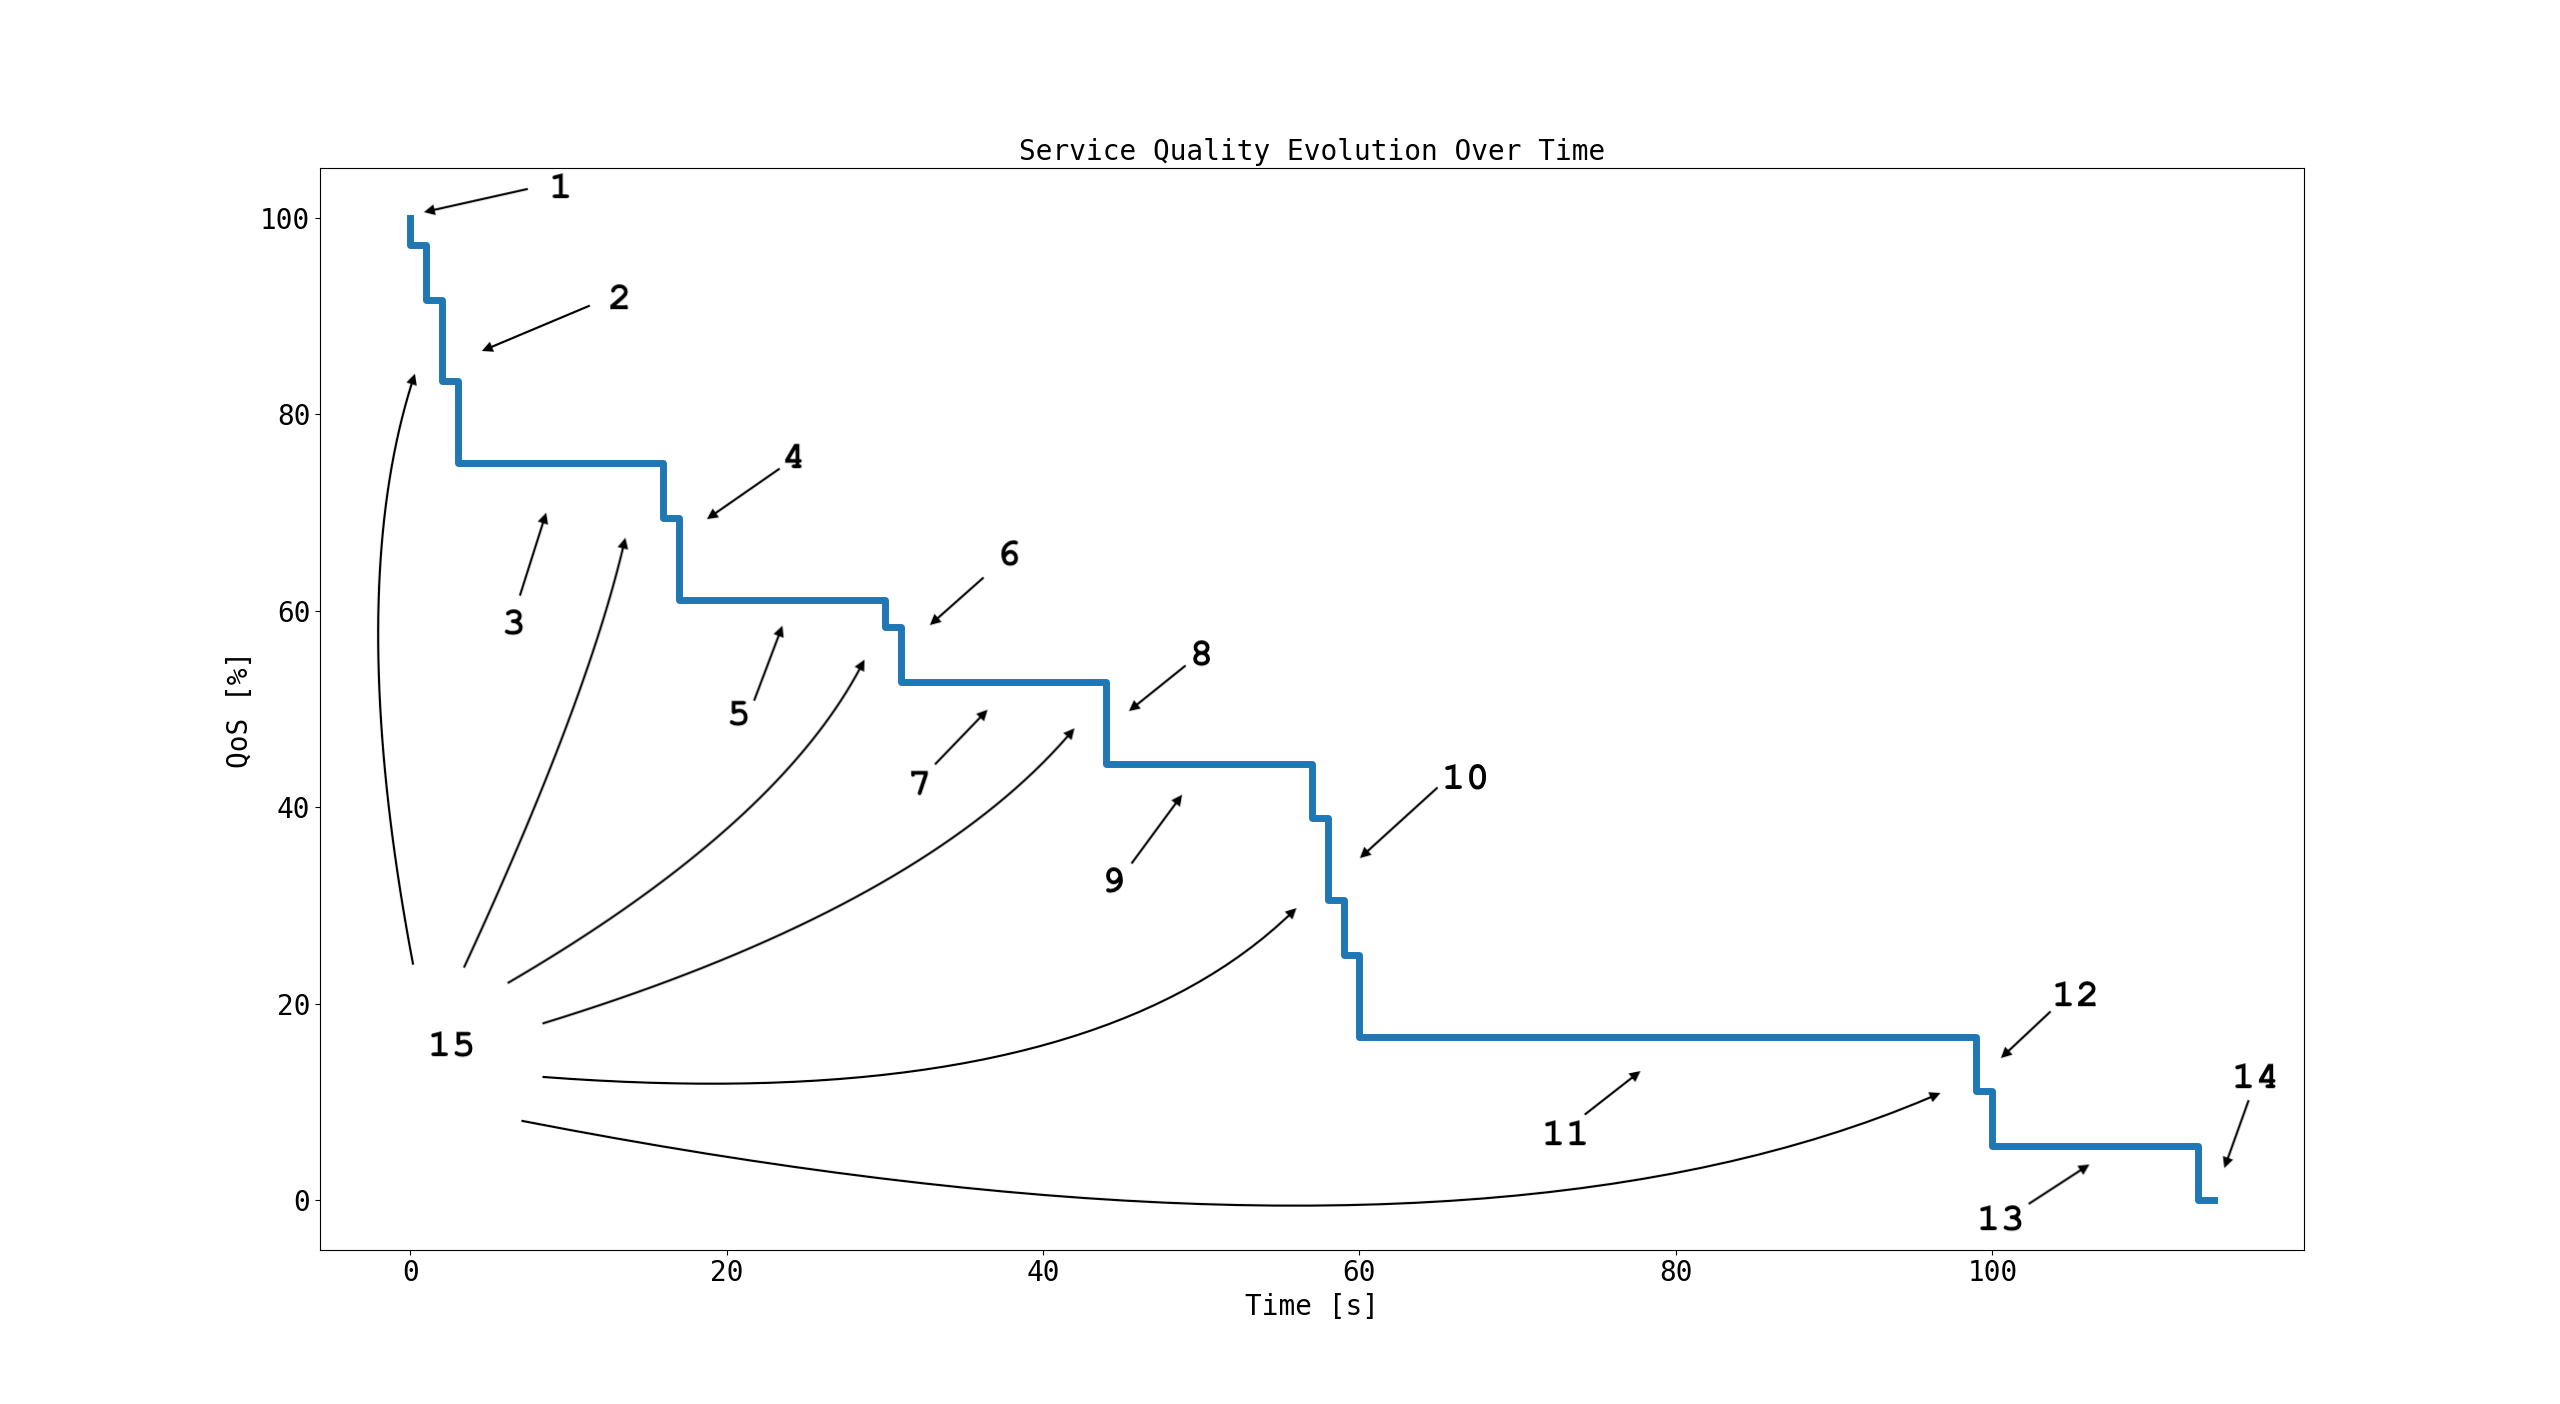
\includegraphics[width=\linewidth]{atk_static_net.png}
                \caption[\textit{QoS} on a Static Topology]{Evolution of the \textit{QoS} Over Time for a Static Topology.}
                \label{fig:static-atk}
            \end{sidewaysfigure}

            \begin{sidewaysfigure}
                \centering
                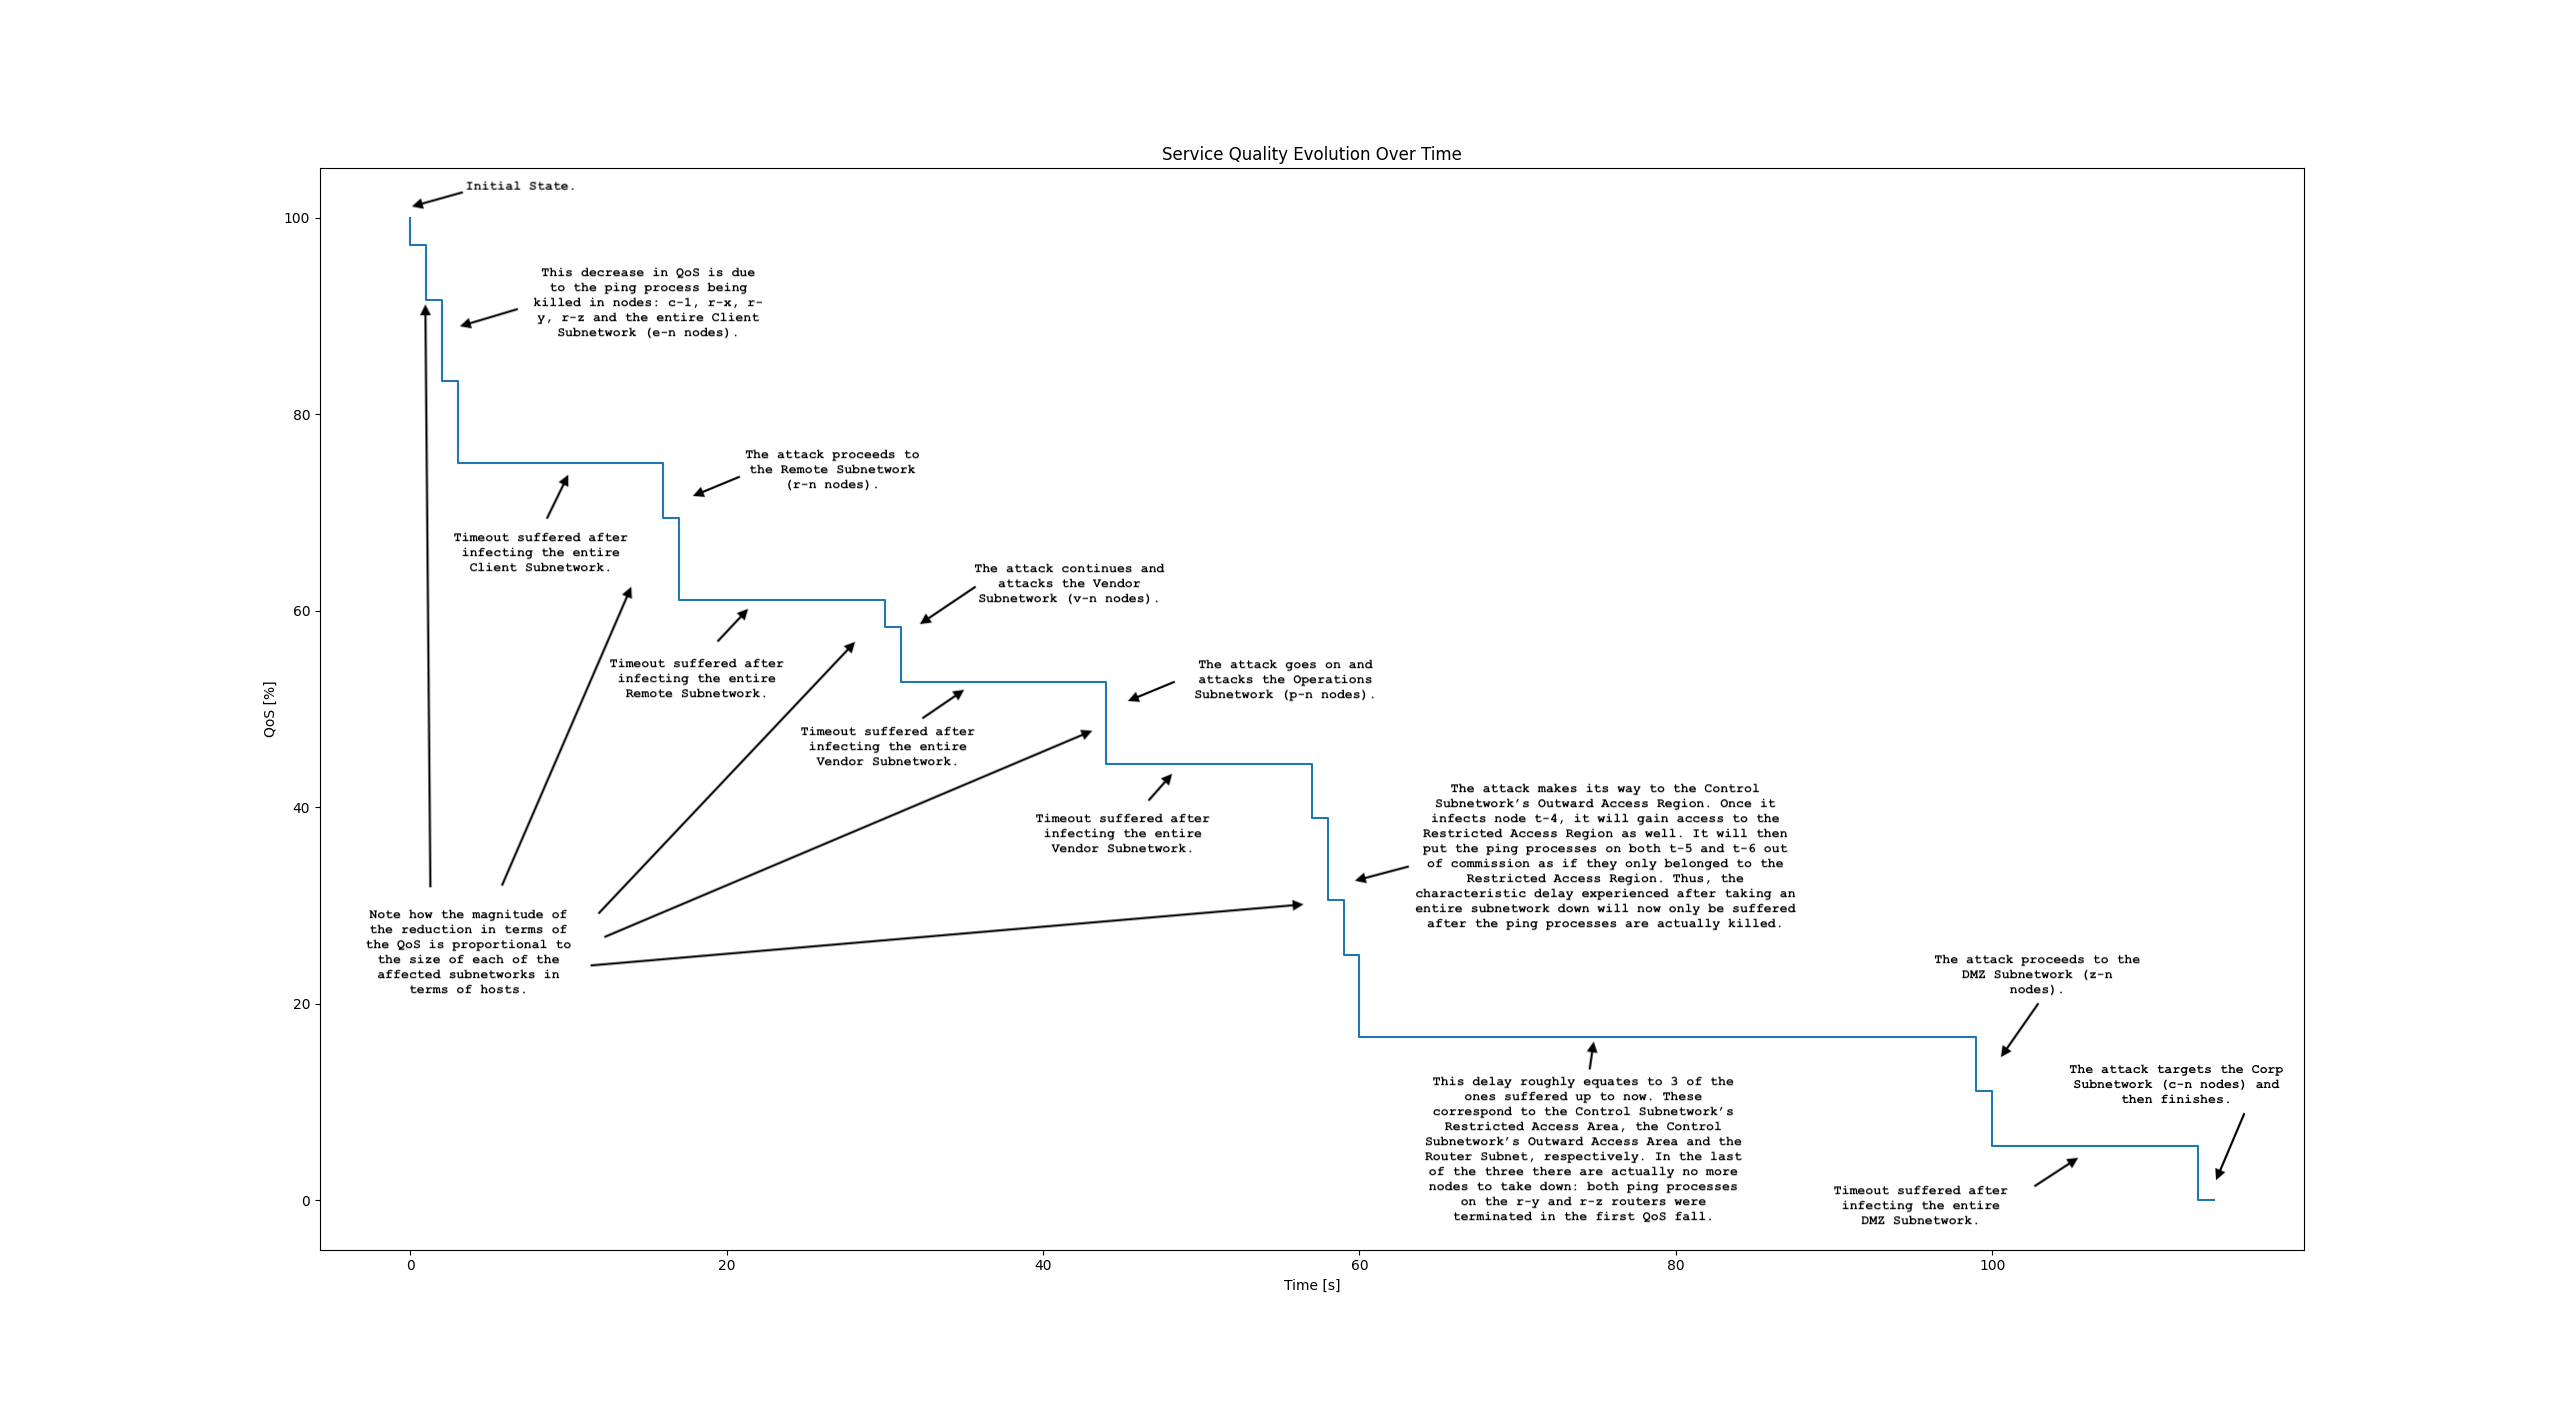
\includegraphics[width=\linewidth]{atk_static_net_annotated.png}
                \caption[Annotated \textit{QoS} on a Static Topology]{Annotated Evolution of the \textit{QoS} Over Time for a Static Topology.}
                \label{fig:static-atk-annotated}
            \end{sidewaysfigure}

            \begin{sidewaysfigure}
                \centering
                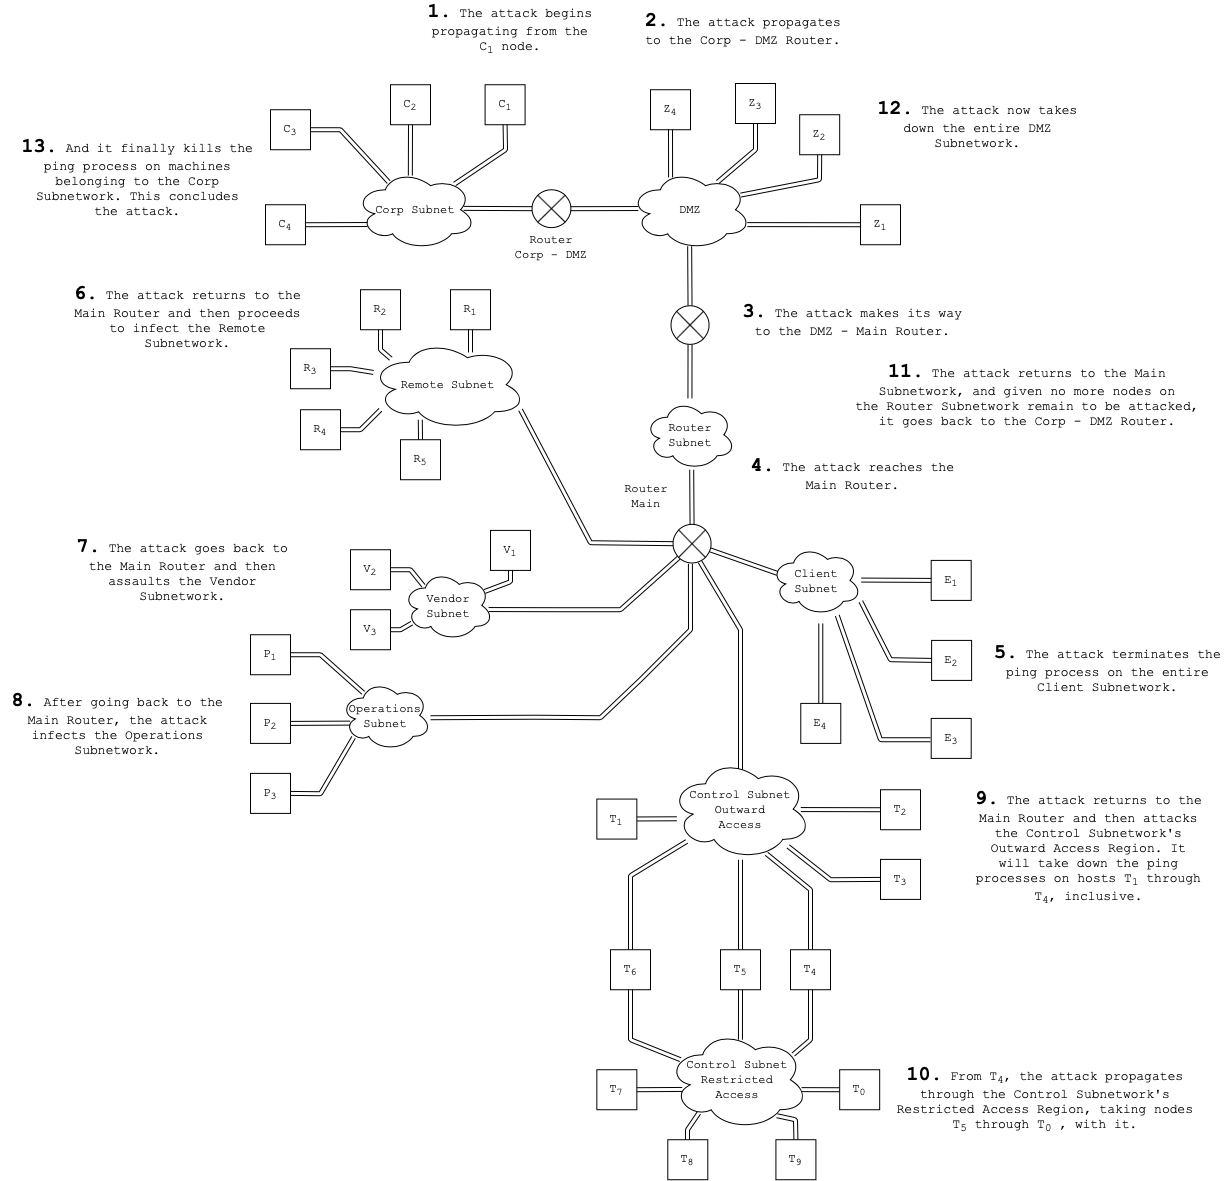
\includegraphics[width=\linewidth]{atk_progression.png}
                \caption[Attack Progression]{Attack Progression Over the Network.}
                \label{fig:atk-progression}
            \end{sidewaysfigure}

            \lstinputlisting[language = bash, caption = Retrieved Data Points for the Attack on a Static Network., label = lst:static-atk]{Experiment_data/atk-static-net.csv}

        \subsection{Trying to Mitigate the Attack}
            Given the contents of figure \ref{fig:atk-evolution} we are certain that the last hosts that are to be attacked are $C_2 \to C_4$. We can then try to move several other hosts to the \textit{Corp Subnetwork} (figure \ref{fig:top-ics}) so that they suffer the attack's consequences at a later time than they normally would. Given the ``virus'' will still be subject to a delay after sweeping each subnetwork, this strategy should provide a bit of leeway for the hosts we are to move.\\

            In order to run this experiment we defined the \texttt{mitigate-atk} command on top of those already discussed on section \ref{sec:cli-cmds}. It will basically call the \texttt{mvnode} command repeatedly and move the following hosts to the \textit{Corp Subntework}: $E_1 \to E_4;\ R_1 \to R_5;\ V_1 \to V_3;\ P_1 \to P_3$. We decided to add this auxiliary order due to the speed with which the attack propagates. If we were to manually move the $15$ nodes we would be tarnishing the data, making it harder to interpret in a satisfactory manner. Then, after launching the attack exactly as described in the previous section we issue the \texttt{mitigate-atk} command, thus triggering the movement of the nodes we have just specified. As soon as said order is invoked we need not do anything more: we will gather the data through the \texttt{dumpt-atk-data} once it has terminated. The data we gathered and then used to draw the plots is included on listing \ref{lst:dynamic-atk}\\

            Given the ``manual'' aspect of having to explicitly issue a command the data presented in this section might not be \textbf{exactly reproducible}. Nonetheless, as long as the user issues the \texttt{mitigate-atk} command in a reasonable time the data should be tremendously similar.\\

            Even though we are moving hosts while the attack is underway, the steps described in figure \ref{fig:atk-progression} are totally applicable: if we regard the network as a collection of subnets its topology \textbf{is not altered} at all by the \texttt{mitigate-atk} command. This explains why the attack's behaviour is the same despite the times at which the events take place not being exactly alike.\\

            Figures \ref{fig:dynamic-atk} and \ref{fig:dynamic-atk-annotated} portray the evolution of the \textit{QoS} when we try to hinder the attack's progress. Figure \ref{fig:atk-comparison} superimposes the evolution of the \textit{QoS} in both cases. Studying it reveals how in the latter case the \textit{QoS} is higher during the entirety of the attack. Thus, we can rest assured our mitigation mechanism is provoking its intended effect.\\

            \begin{sidewaysfigure}
                \centering
                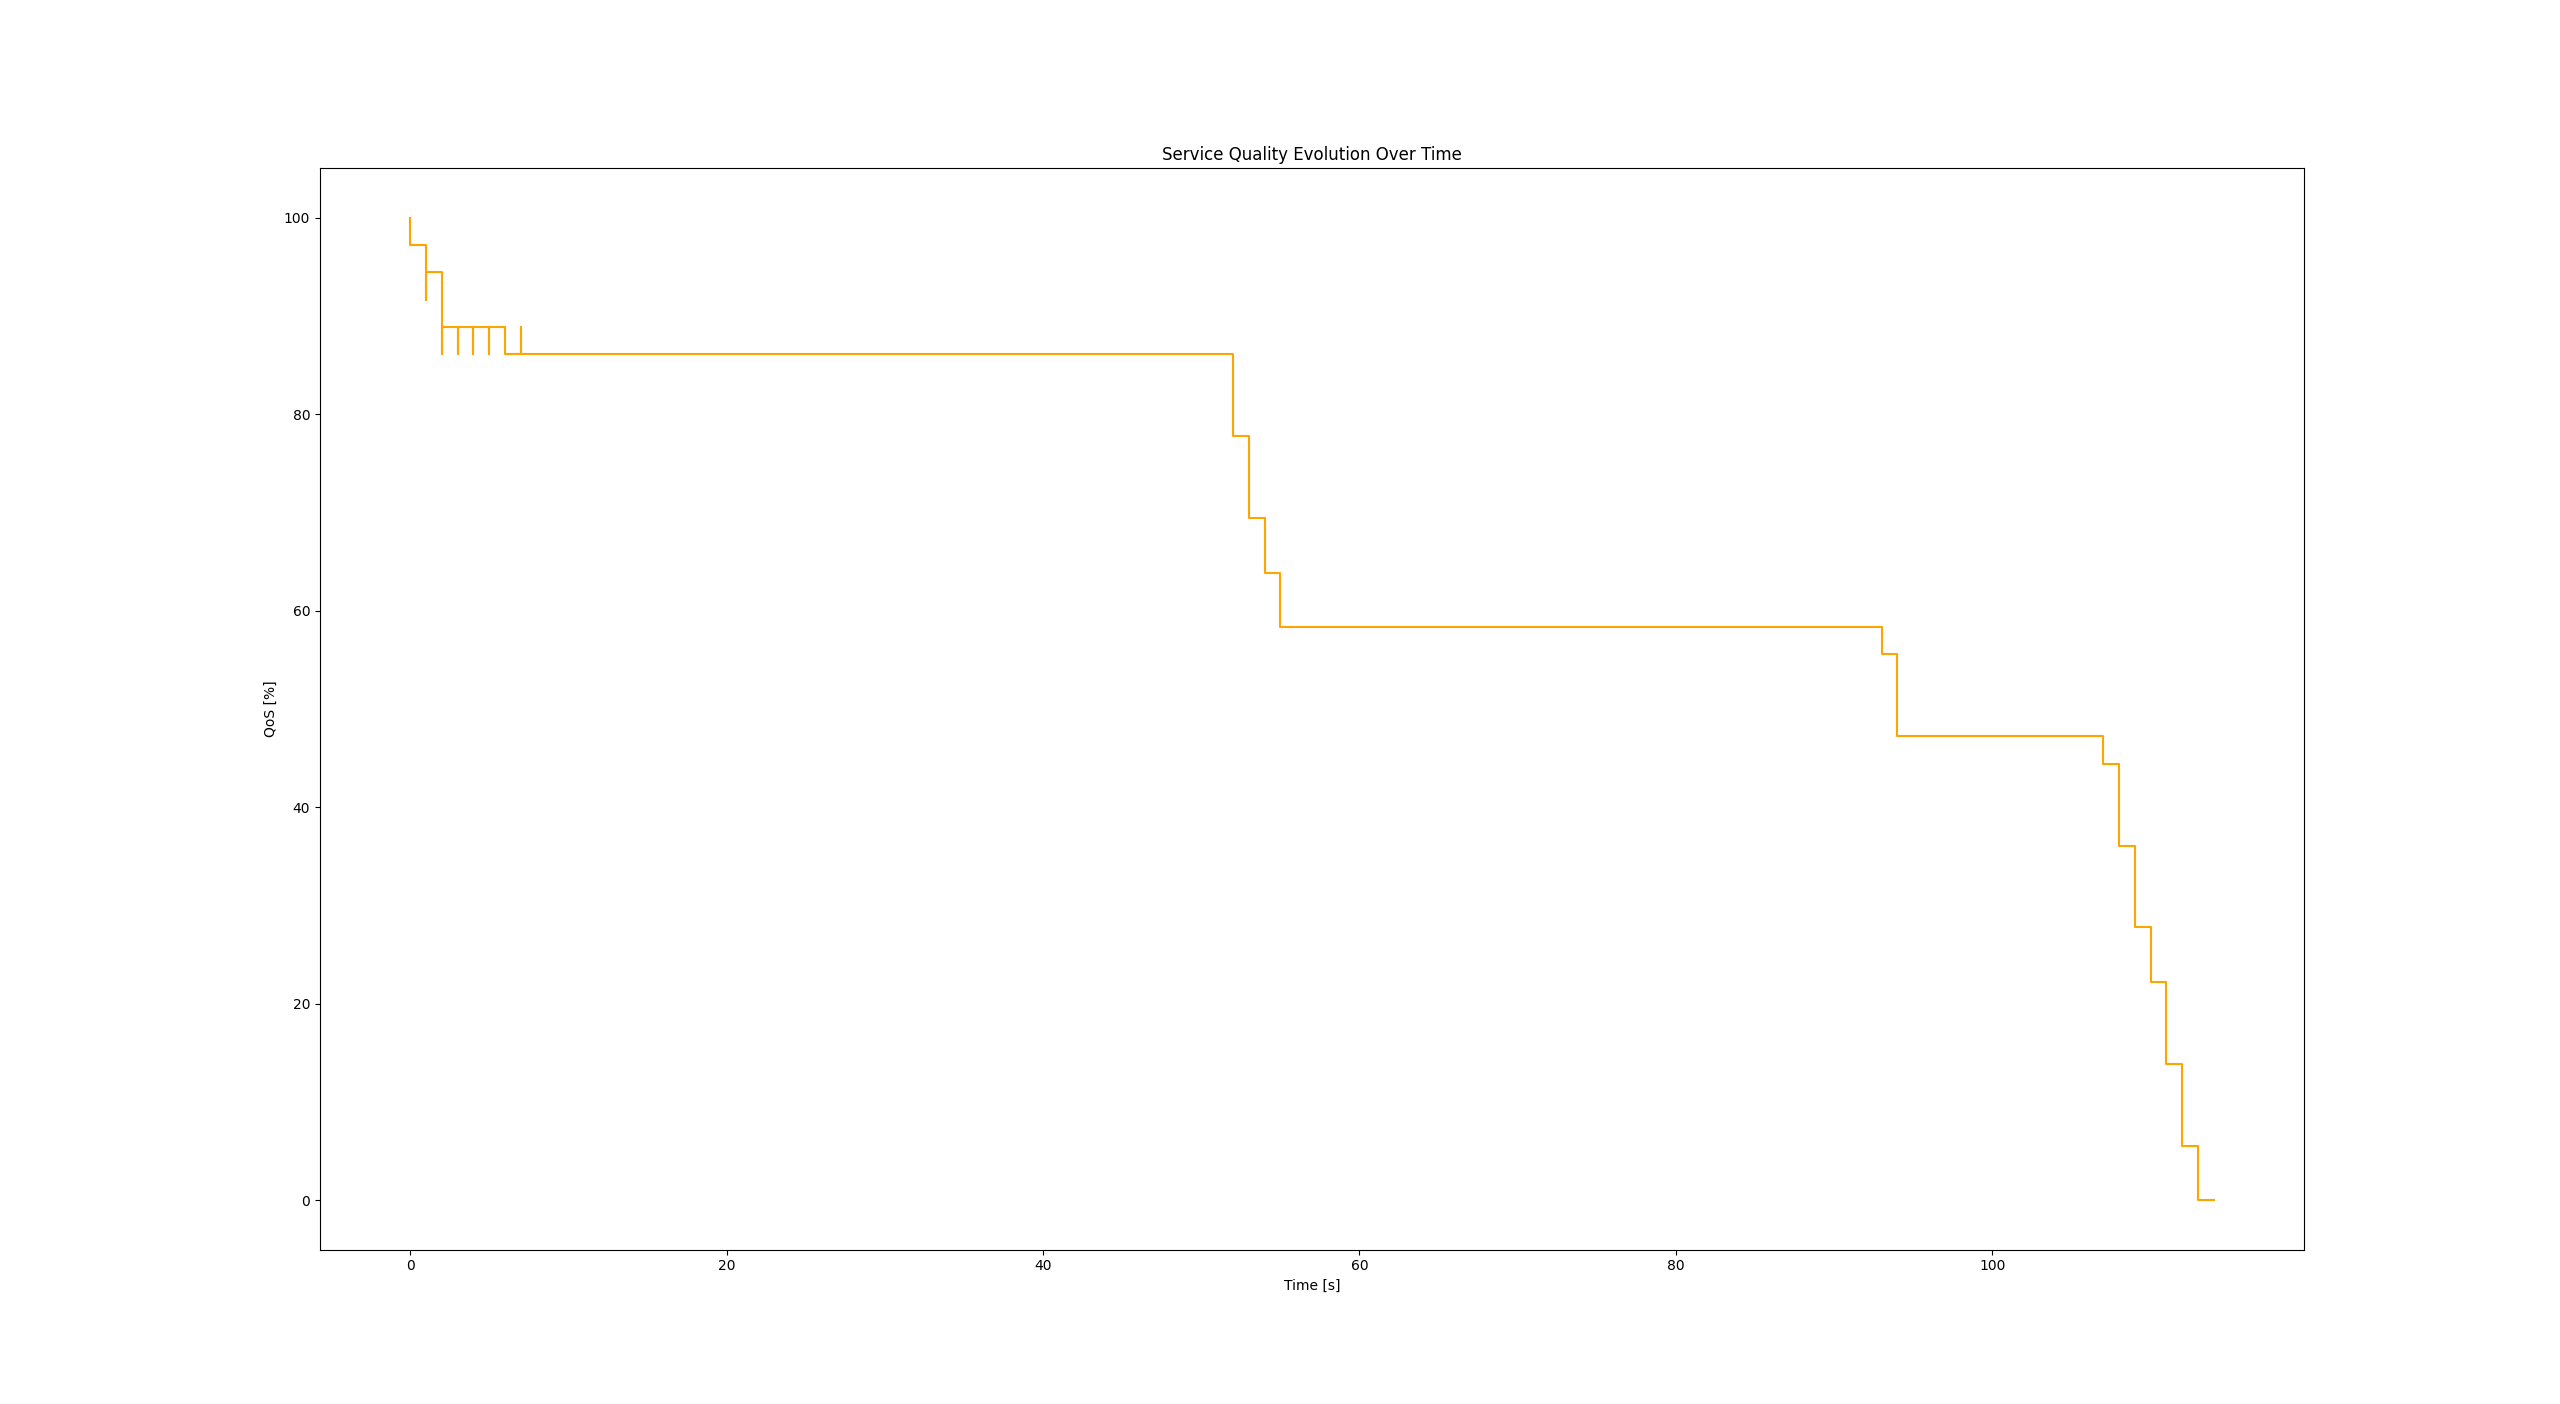
\includegraphics[width=\linewidth]{atk_dynamic_net.png}
                \caption[\textit{QoS} on a Dynamic Topology]{Evolution of the \textit{QoS} Over Time for a Dynamic Topology.}
                \label{fig:dynamic-atk}
            \end{sidewaysfigure}

            \begin{sidewaysfigure}
                \centering
                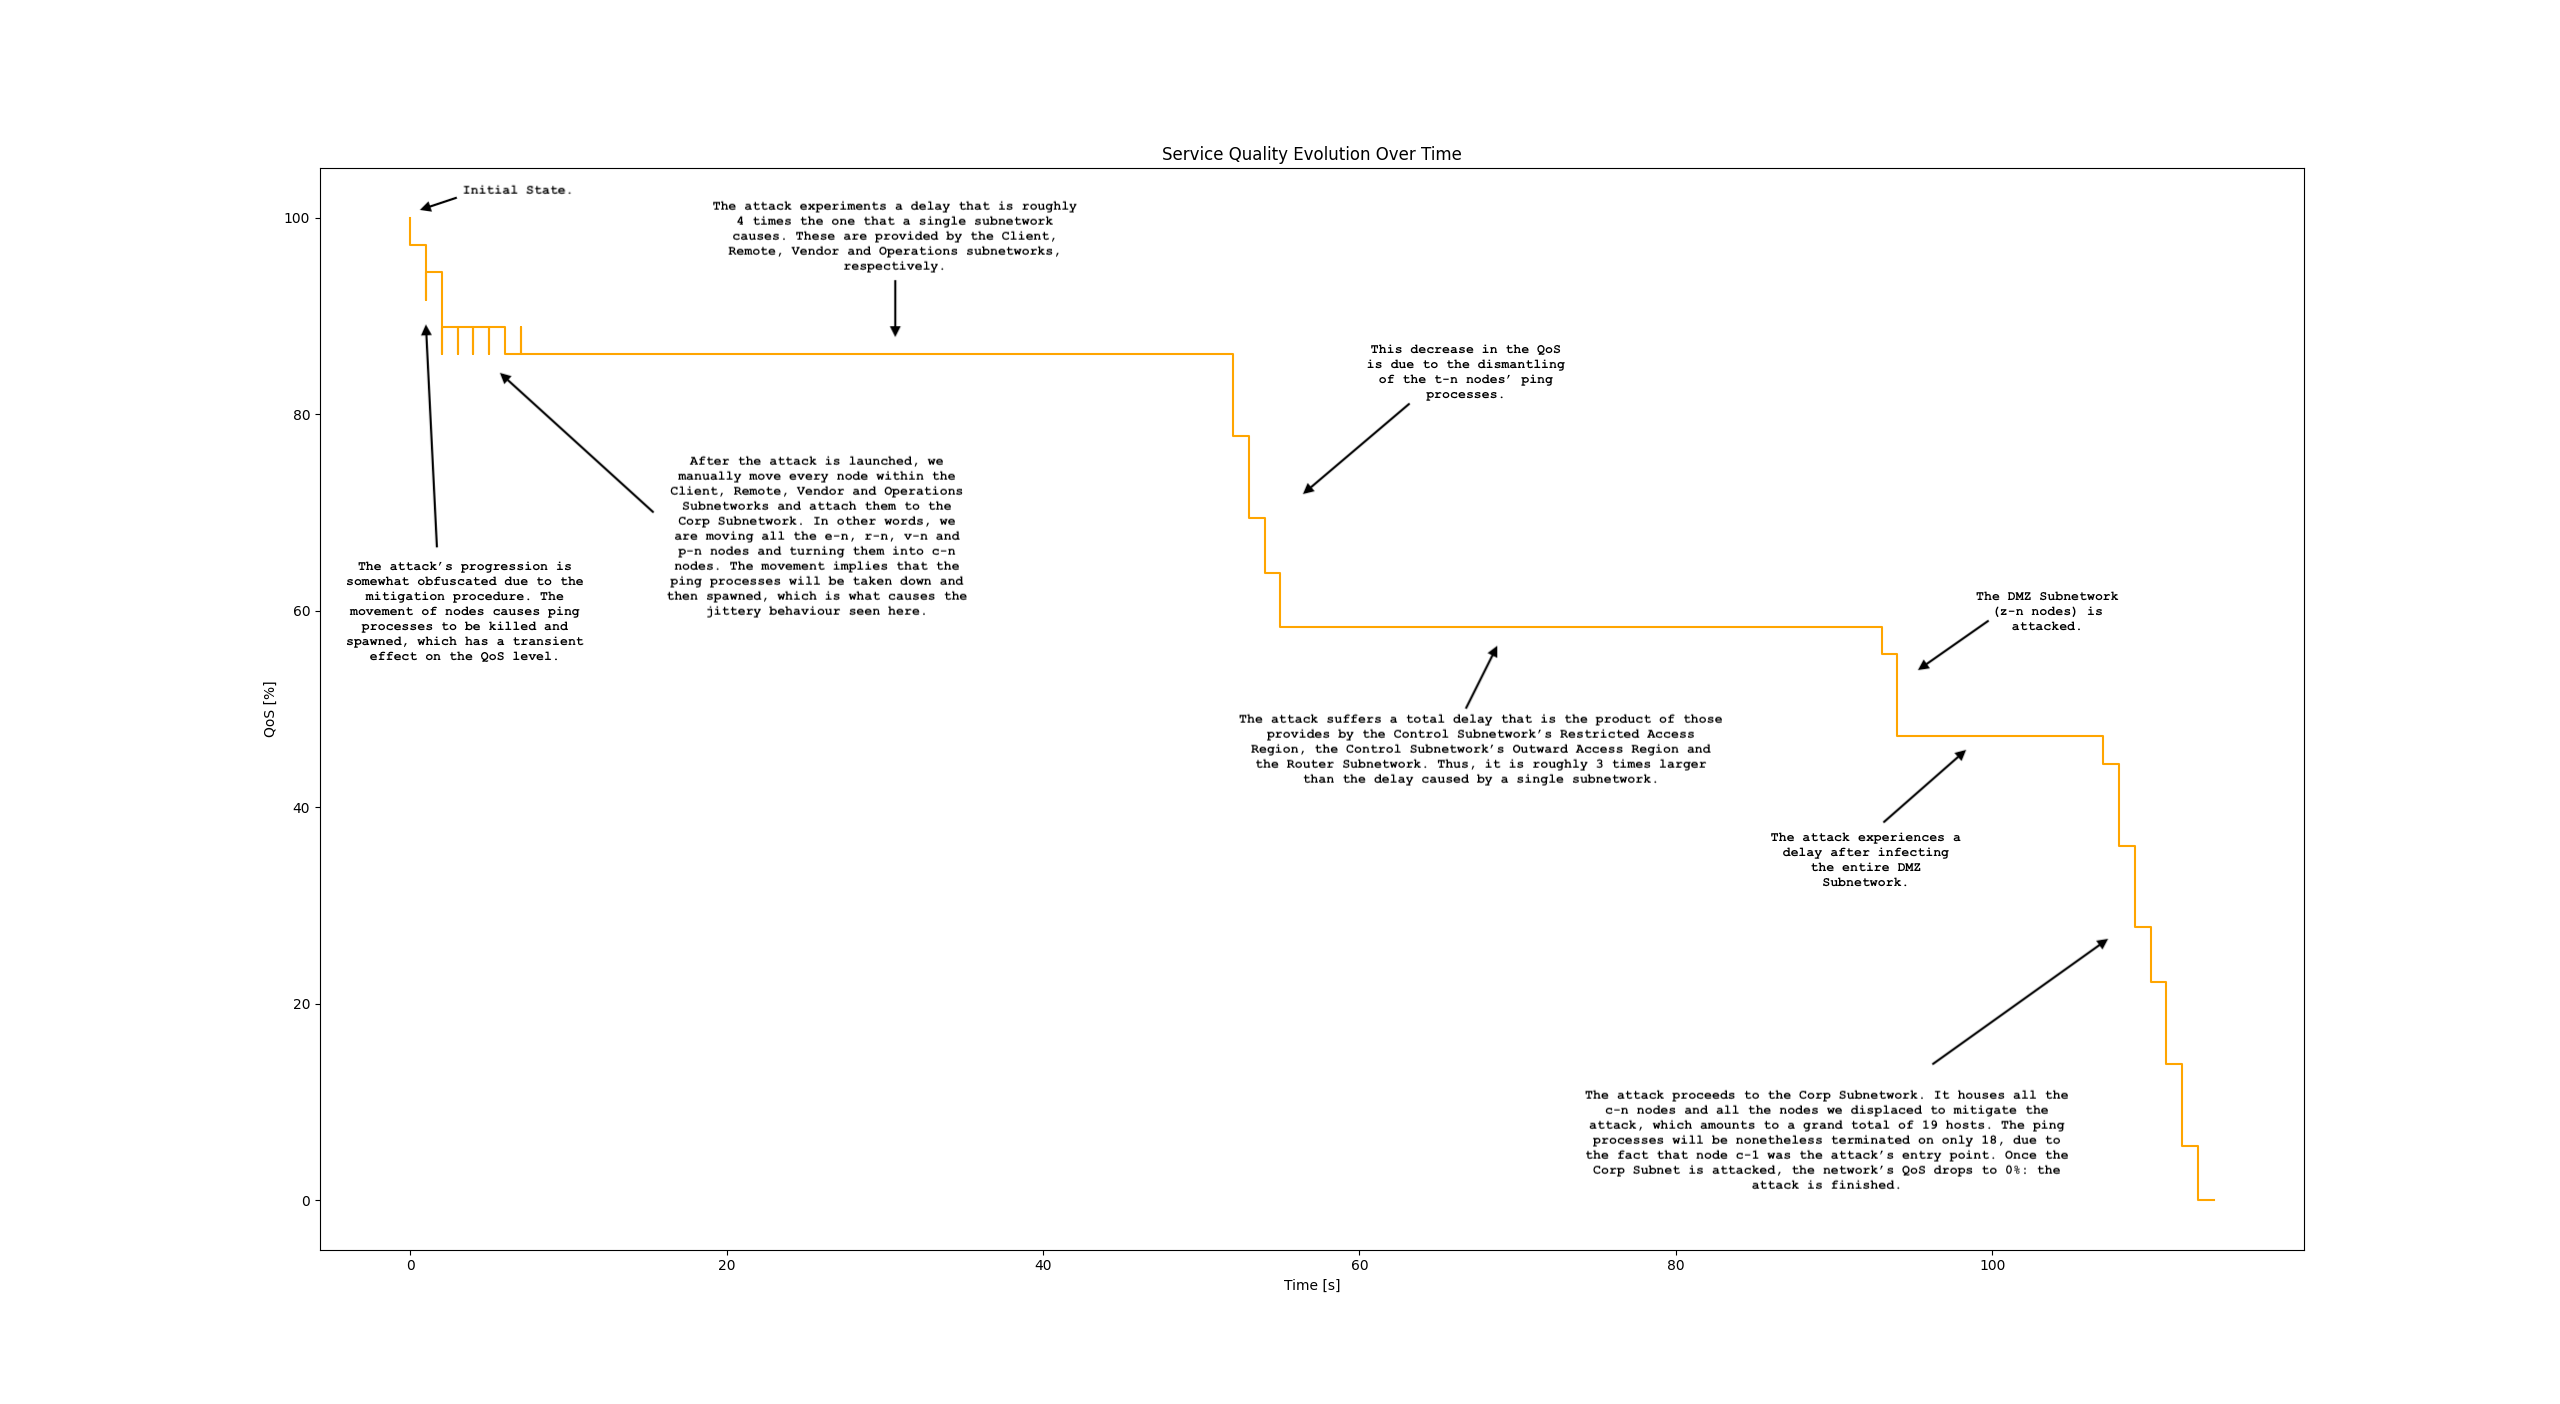
\includegraphics[width=\linewidth]{atk_dynamic_net_annotated.png}
                \caption[Annotated \textit{QoS} on a Dynamic Topology]{Annotated Evolution of the \textit{QoS} Over Time for a Dynamic Topology.}
                \label{fig:dynamic-atk-annotated}
            \end{sidewaysfigure}

            \begin{sidewaysfigure}
                \centering
                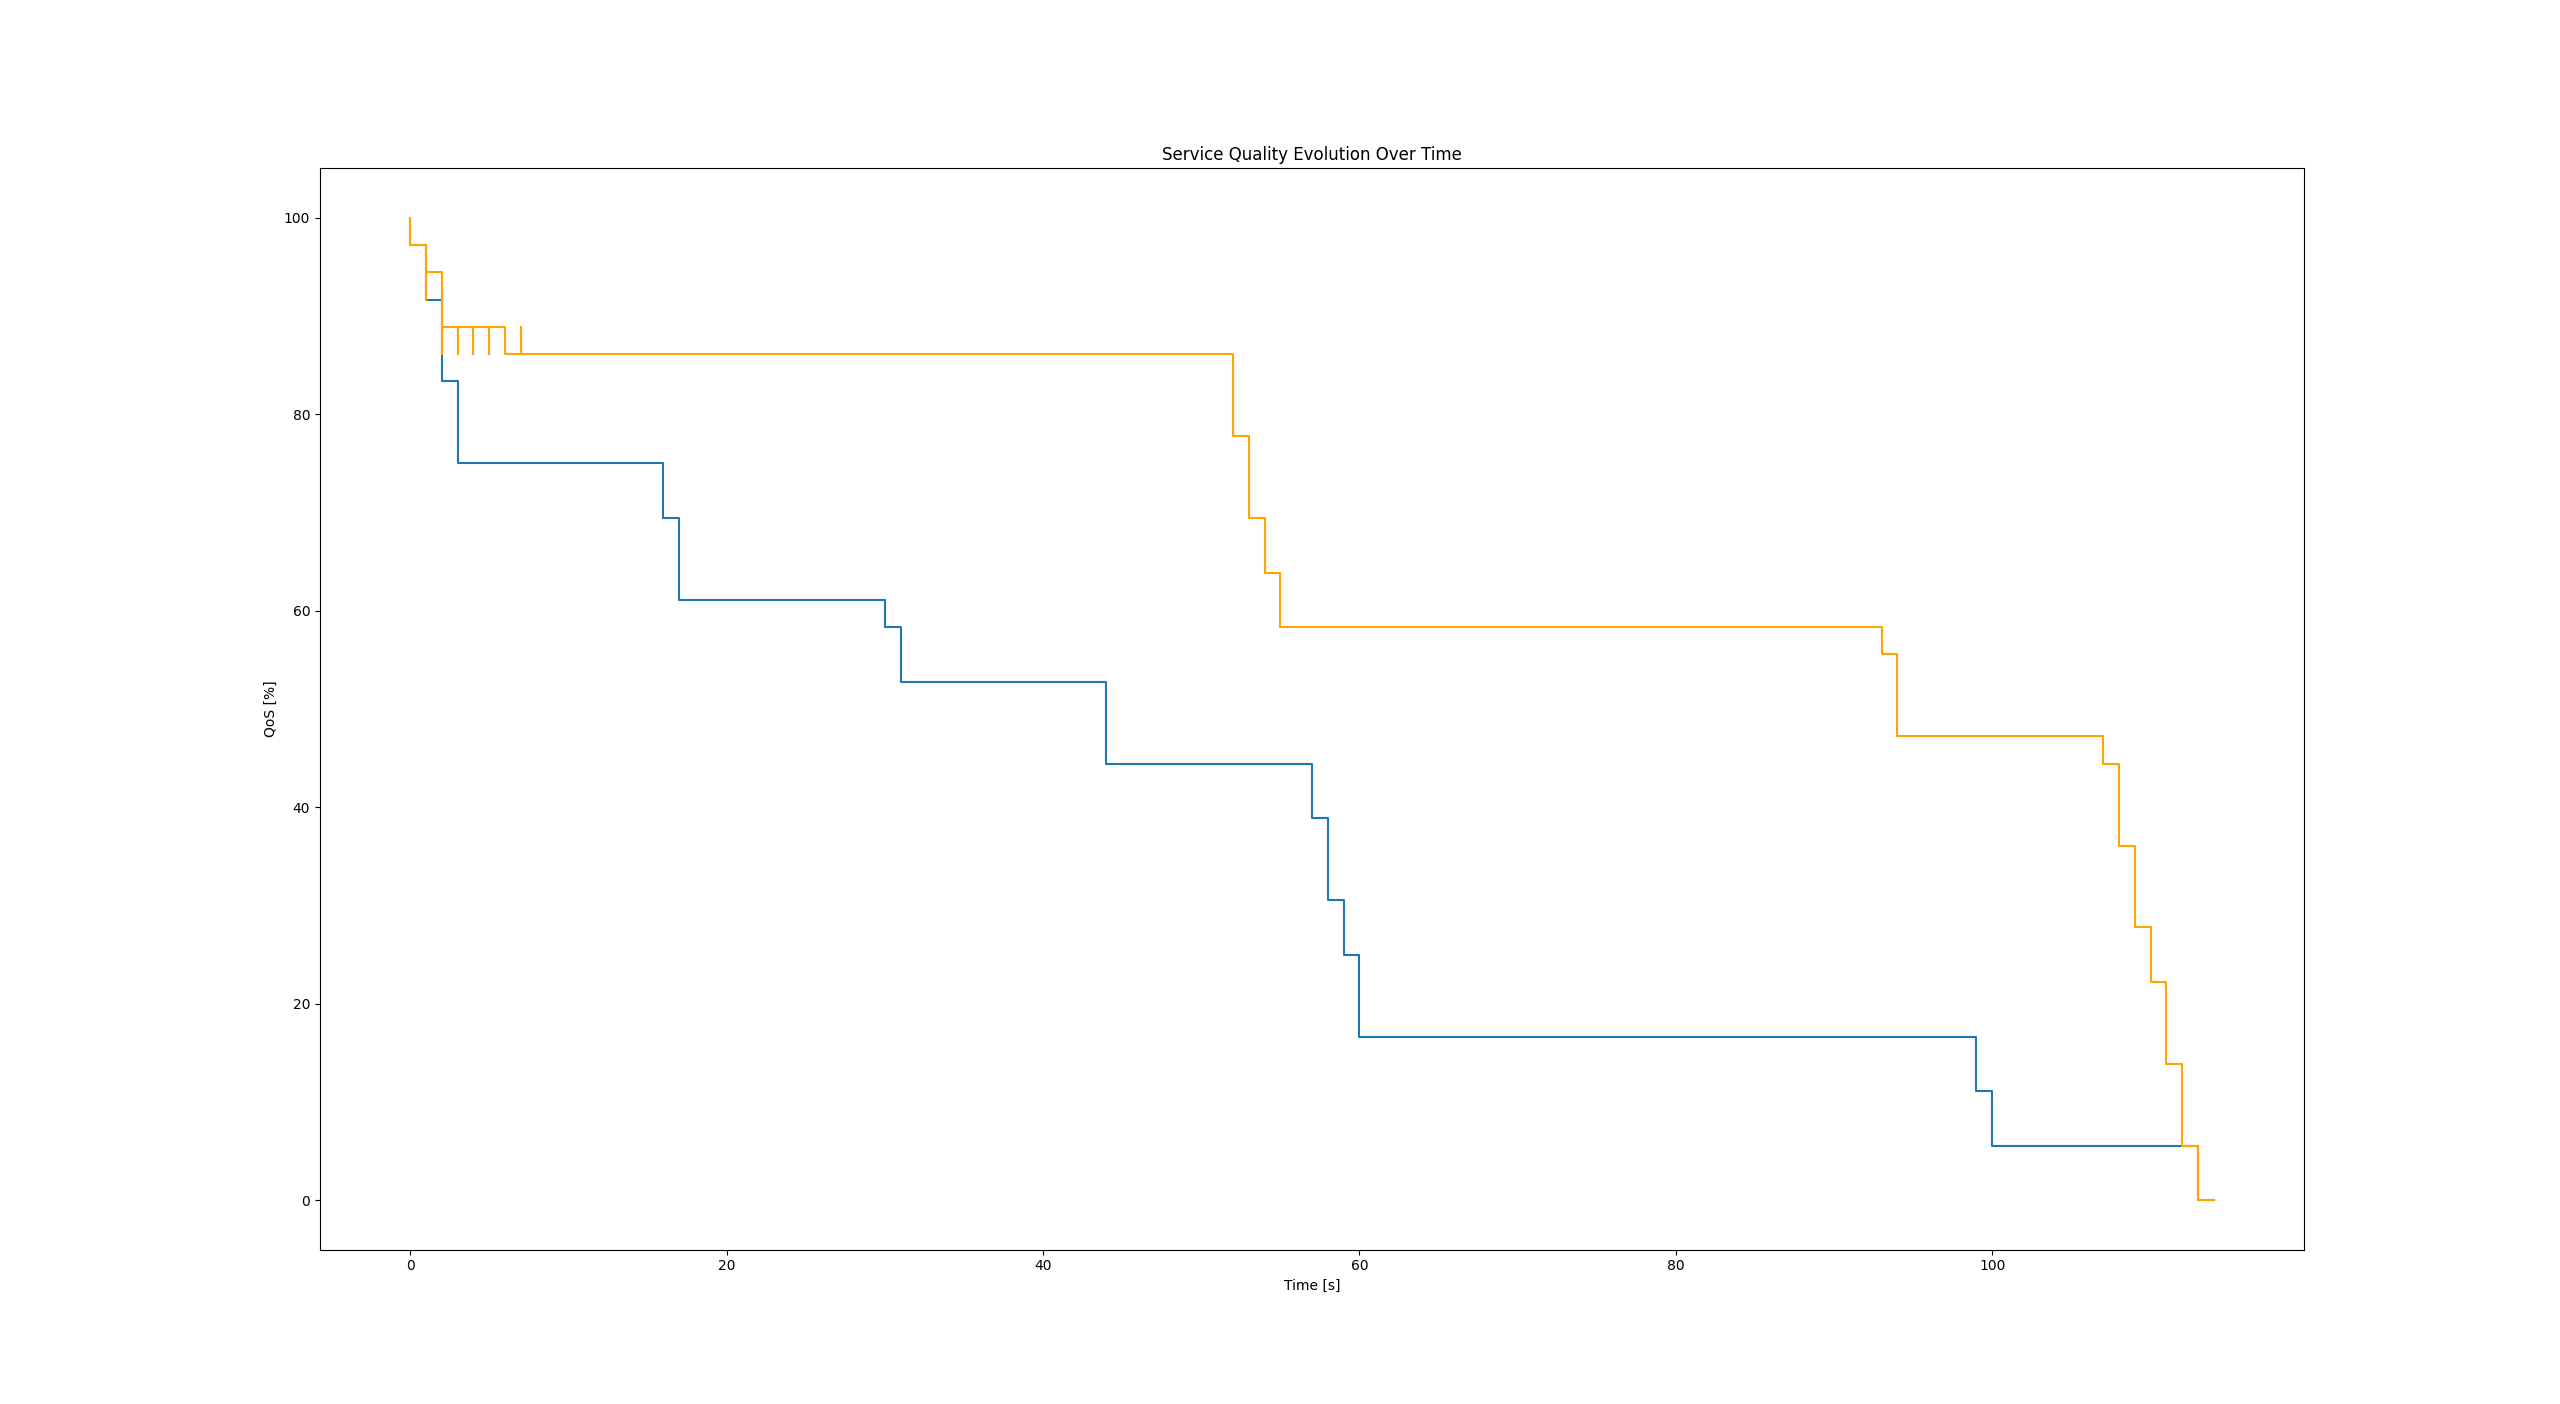
\includegraphics[width=\linewidth]{static_vs_dynamic_atk.png}
                \caption[Attack Mitigation Effect vs. Baseline Case]{Comparison of the Evolution of the \textit{QoS}. \textit{Blue} - Base Case. \textit{Orange} - Mitigated Attack.}
                \label{fig:atk-comparison}
            \end{sidewaysfigure}

            \lstinputlisting[language = bash, caption = Retrieved Data Points for the Attack on a Dynamic Network., label = lst:dynamic-atk]{Experiment_data/mitigated-atk.csv}

        The figures we have presented in this section display the evolution of an extremely quick attack. What is more, we have only explored a single quick response to an attack which we have found to be clearly more effective than not taking any action at all. Nonetheless, the real value of this tool is serving as a testing ground for more complex and efficient techniques that are being developed as part of associated research projects. We have decided to prepare this short demonstration in an effort to showcase our tool's potential and we have not even scratched the surface.\\
